\section{Introduzione}
Il programma realizzato permette di gestire utenti e interventi di una squadra della Protezione Civile, utilizzando una semplice interfaccia grafica realizzata tramite il framework Qt.
In particolare, gli utenti sono suddivisi in base al loro ruolo:
\begin{itemize}
	\item volontario;
	\item caposquadra;
	\item amministratore.
\end{itemize}
Ogni utente, in base al proprio ruolo, avrà accesso a particolari funzionalità quali aggiungere o cancellare un utente nel sistema, visualizzare gli utenti della propria squadra, visualizzare e pianificare interventi. A differenza degli amministratori, il volontario e il caposquadra appartengono a una squadra, caratterizzata da un nome e da un'area di intervento. 
Per accedere all'applicazione è necessario effettuare un login, inserendo uno username, rappresentato dal proprio numero di matricola e una password scelta al momento della registrazione dell'utente.
L'interfaccia grafica è stata realizzata attraverso gli oggetti QtWidget che permettono di semplificare la realizzazione della GUI tramite l'editor Qt Creator.

\section{Funzionamento}
All'avvio del programma, viene subito richiesto di effettuare il login (\Fig\ref{fig:loginform}), inserendo lo username (costituito dalla matricola assegnata dal sistema al momento dell'inserimento dell'utente) e la password. In caso di username e/o password errati, viene mostrato un messaggio di errore e cancellati lo username e la password errati. Non è quindi possibile procedere oltre nell'applicazione.

\begin{figure}[h!]
	\centering
	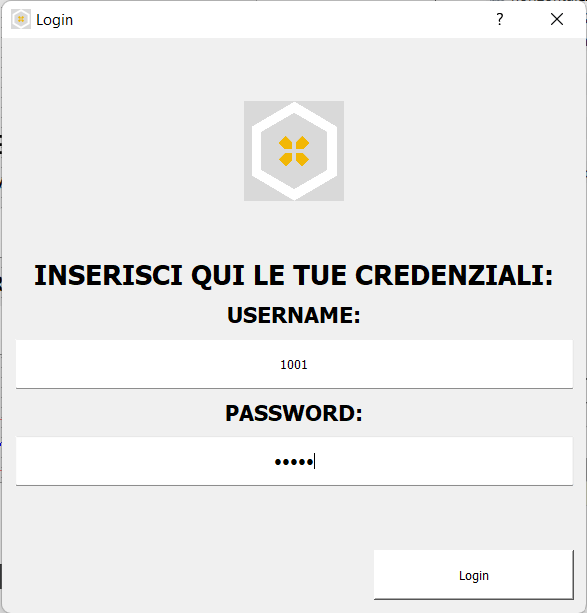
\includegraphics[width=0.4\linewidth]{./ImageFiles/loginform}
	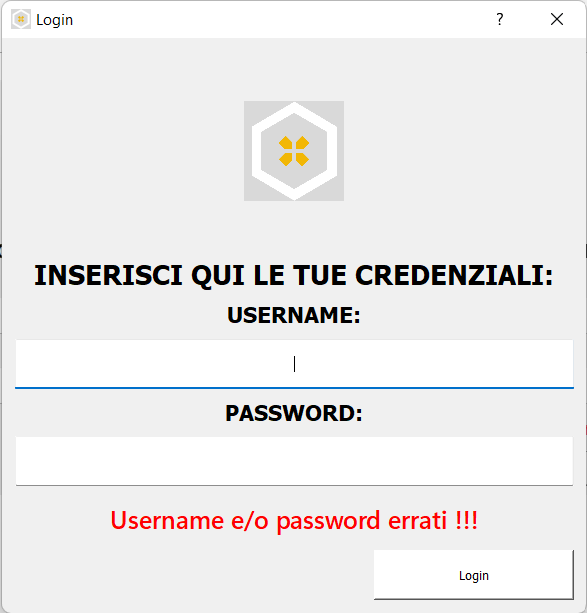
\includegraphics[width=0.4\linewidth]{./ImageFiles/loginform_errato}
	\caption{Finestra di login e login errato.}
	\label{fig:loginform}
\end{figure}

Al contrario, se le credenziali di accesso sono corrette viene mostrato all'utente la schermata principale (\Fig\ref{fig:home_foreman}). La schermata principale è divisa in due sezioni. Nella parte sinistra è possibile vedere tutte le informazioni memorizzate dell'utente (fotografia, matricola, nome, cognome, data di nascita, email, numero di telefono, sesso) e le informazioni relative alla squadra (identificativo e nome della squadra, nome e coordinate dell'area di intervento). Le informazioni relative alla squadra non sono mostrate nel caso in cui l'utente sia un amministratore, in quanto non appartenente a nessuna squadra.

\begin{figure}[h!]
	\centering
	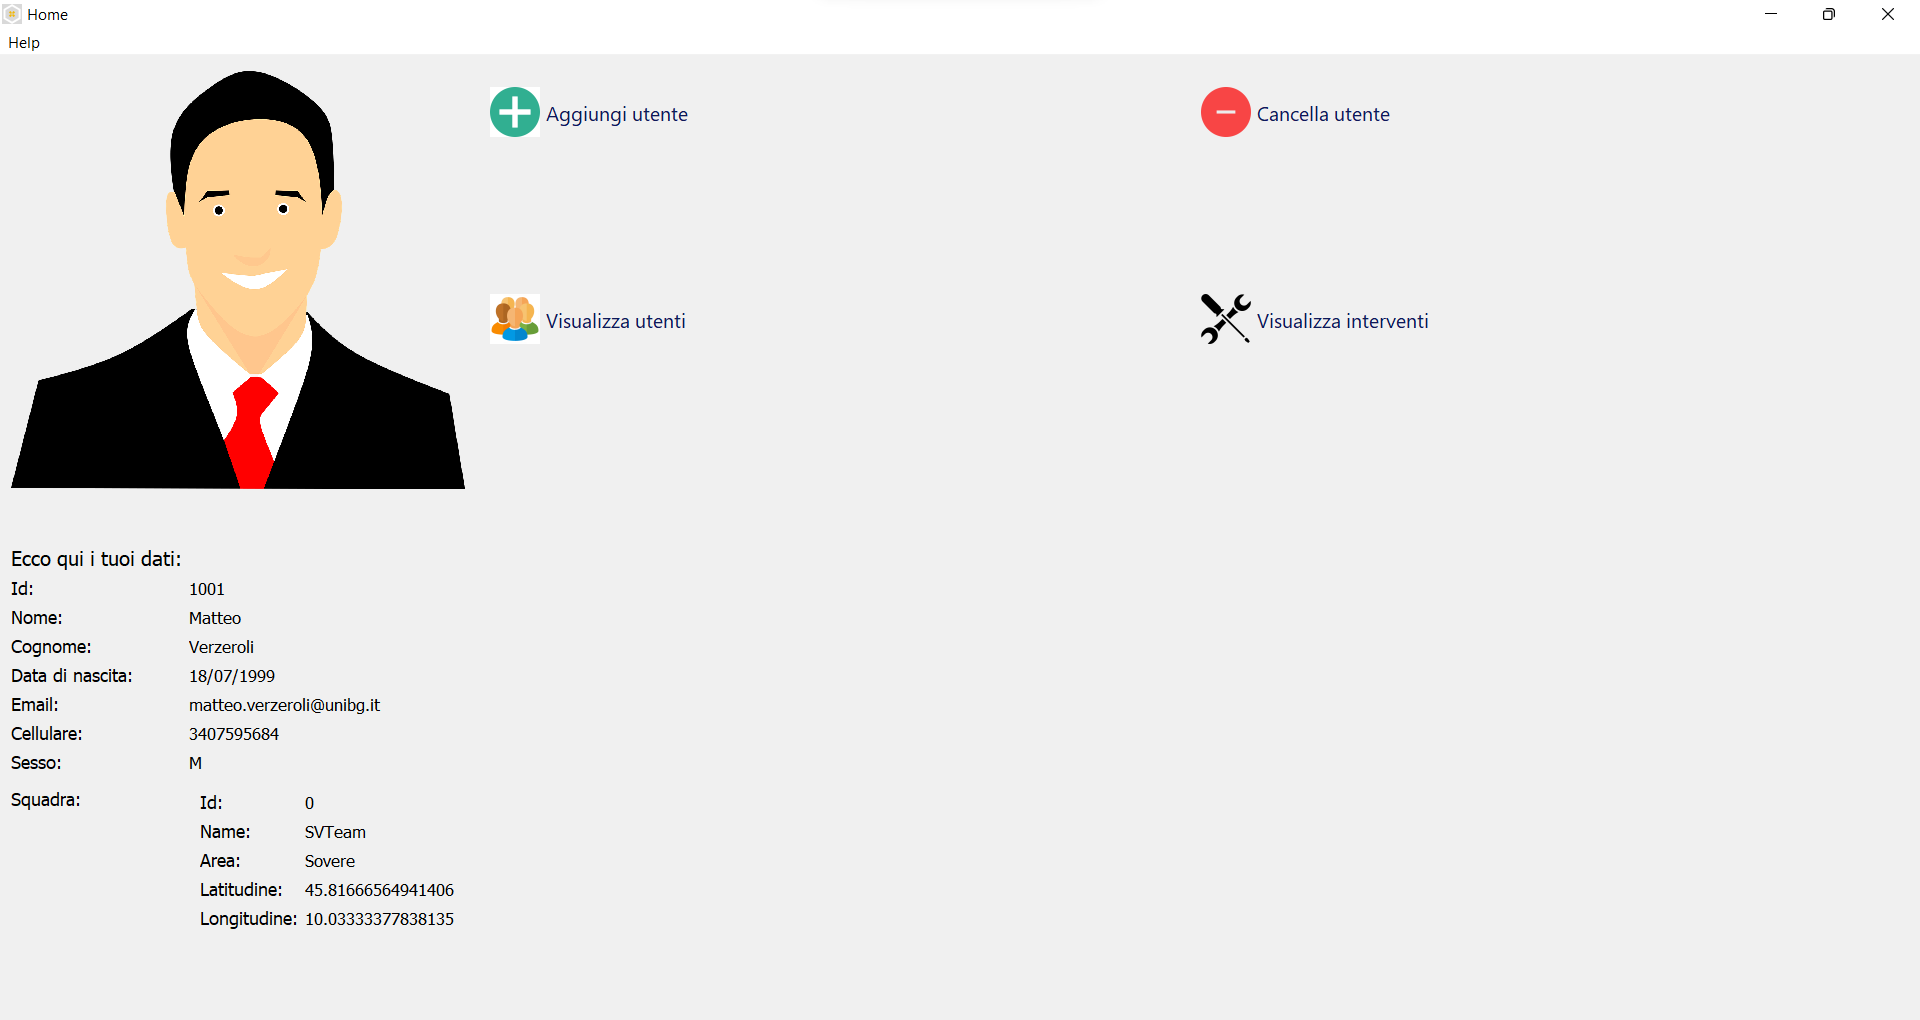
\includegraphics[width=1\linewidth]{./ImageFiles/home_foreman}
	\caption{Finestra principale di un caposquadra.}
	\label{fig:home_foreman}
\end{figure}

Nella parte destra è possibile vedere un piccolo menù dalla quale scegliere le operazioni da eseguire: aggiungere un utente, eliminare un utente, visualizzare gli utenti e gli interventi. A seconda del ruolo dell'utente loggato, questo menù mostrerà diverse opzioni. In particolare, al volontario è permesso solamente visualizzare gli interventi, mentre all'amministratore non è possibile visualizzare gli interventi. Cliccando un pulsante nel menù sarà possibile eseguire le operazioni richieste.

\subsection{Inserimento nuovo utente}
Cliccando su \textit{Aggiungi utente} viene visualizzata una form da compilare per inserire i dati dell'utente da inserire, come mostrato nella \Fig\ref{fig:new_user}. 
\begin{figure}[h!]
	\centering
	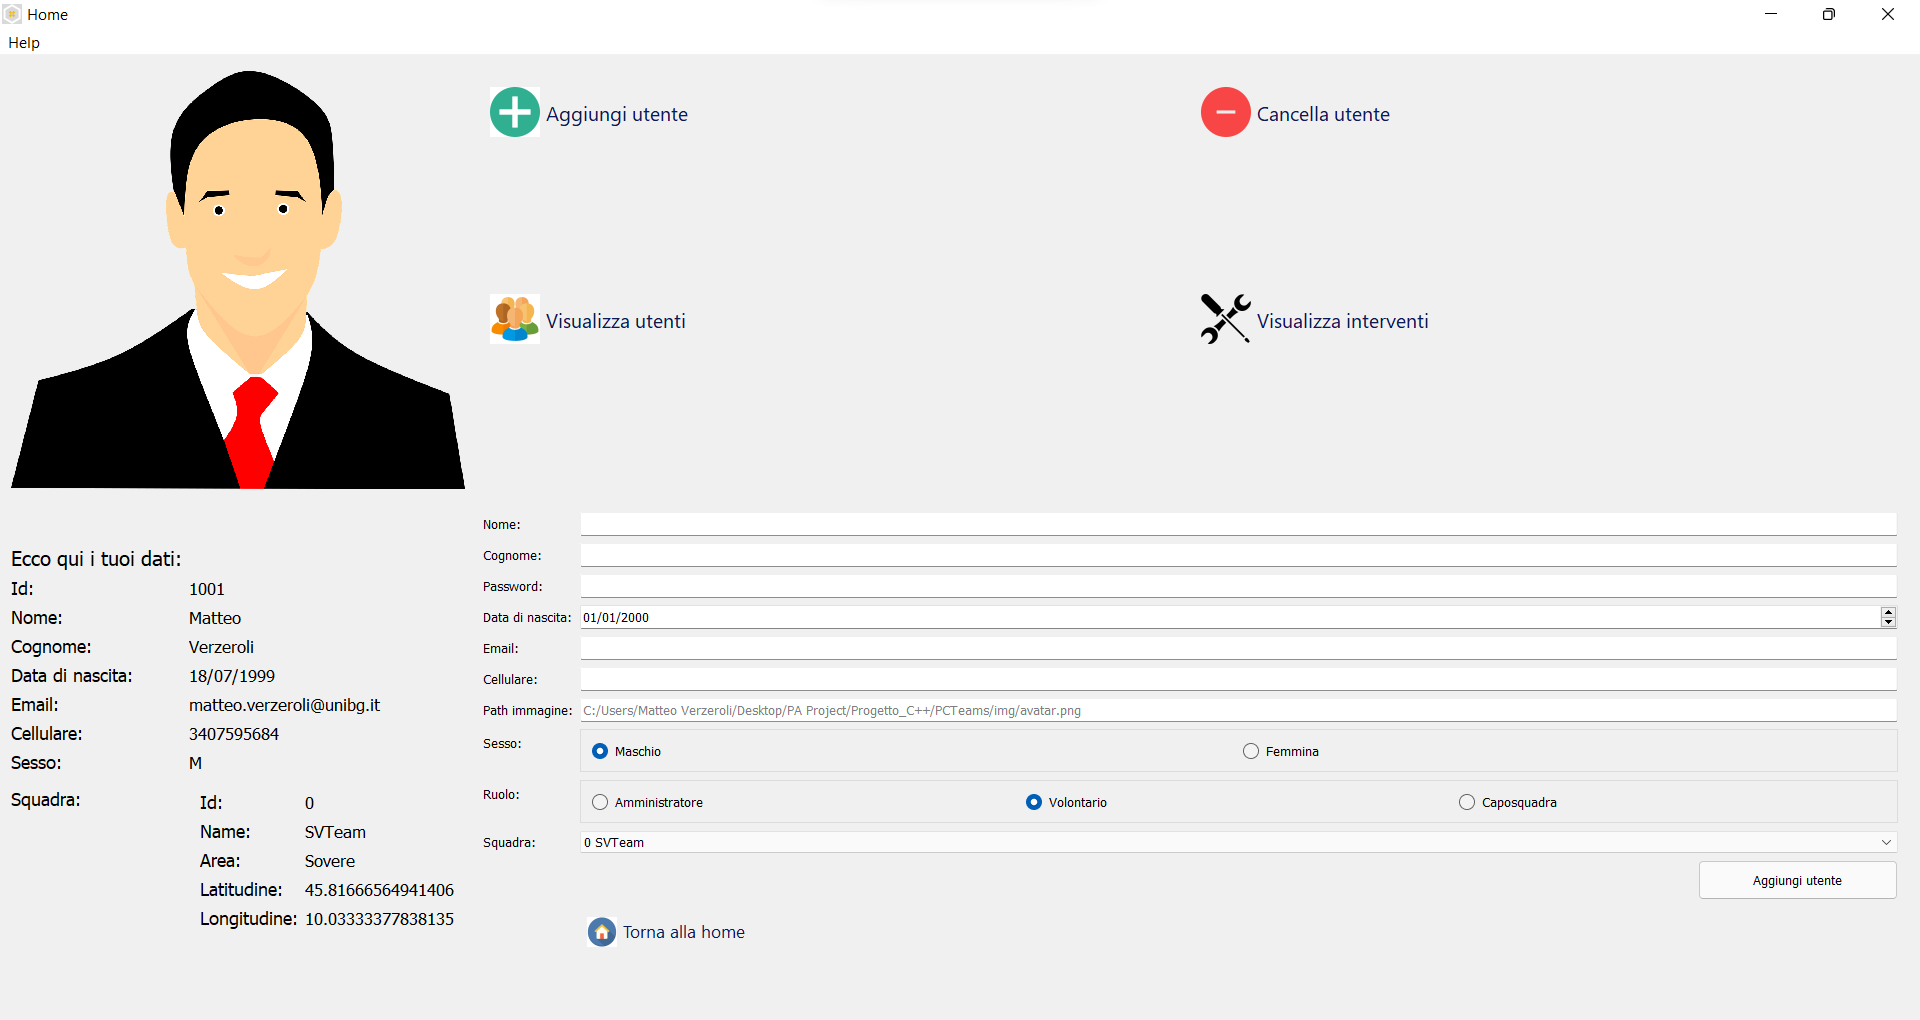
\includegraphics[width=1\linewidth]{./ImageFiles/new_user}
	\caption{Inserimento nuovo utente.}
	\label{fig:new_user}
\end{figure}

Si noti in particolare che bisogna anche indicare il ruolo. Se viene cliccato il ruolo \textit{Volontario} oppure \textit{Caposquadra}, viene mostrato anche una \textit{combo box} nella quale è possibile scegliere una squadra in cui inserire un utente.

Nel caso in cui si voglia inserire un volontario, le squadre selezionate vengono così selezionate: 
\begin{itemize}
	\item se l'utente attualmente loggato è un amministratore, vengono mostrate tutte le squadre inserite nel sistema;
	\item se l'utente attualmente loggato è un caposquadra, viene mostrata solamente la propria squadra.
\end{itemize}
Invece, se si vuole inserire un caposquadra vengono mostrate tutte le squadre inserite nel sistema che non hanno ancora un caposquadra.
Premendo il pulsante \textit{Inserisci utente}, l'utente viene inserito nel sistema e viene mostrato un messaggio di conferma nella \textit{status bar} in fondo alla finestra. Se non vengono compilati tutti i campi, il sistema segnala finestra di errore (\Fig\ref{fig:new_user_error}). 

\begin{figure}[h!]
	\centering
	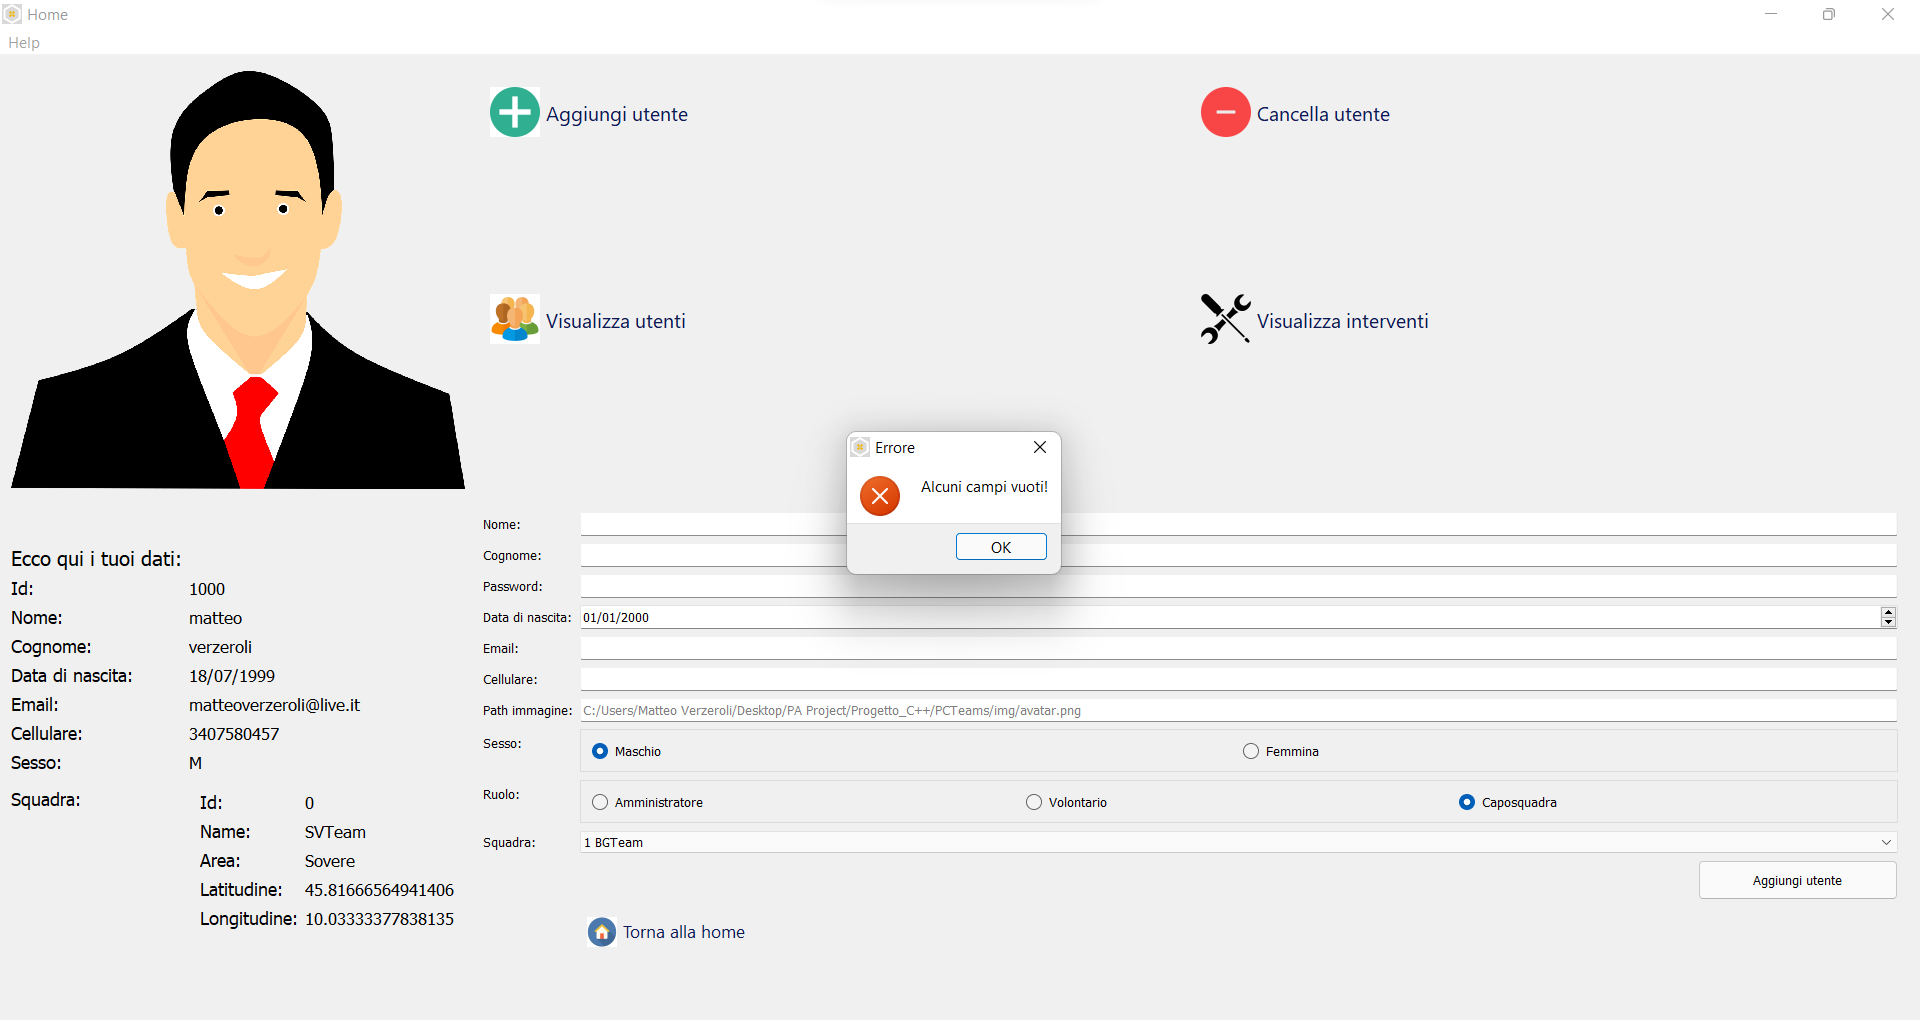
\includegraphics[width=1\linewidth]{./ImageFiles/new_user_error}
	\caption{Errore inserimento nuovo utente.}
	\label{fig:new_user_error}
\end{figure}

\subsection{Cancella utente}
Nel caso in cui si voglia cancellare un utente, è possibile selezionare una squadra (tramite una \textit{combo box}) e indicare l'utente da eliminare, selezionandolo nella lista sottostante (\Fig\ref{fig:delete_user}). Un caposquadra può solamente cancellare utenti della propria squadra. Un amministratore invece può eliminare utenti da tutte le squadre, compresi gli amministratori. Nessuno può eliminare se stesso. Infatti, in tal caso viene mostrato un messaggio di errore.

\begin{figure}[h!]
	\centering
	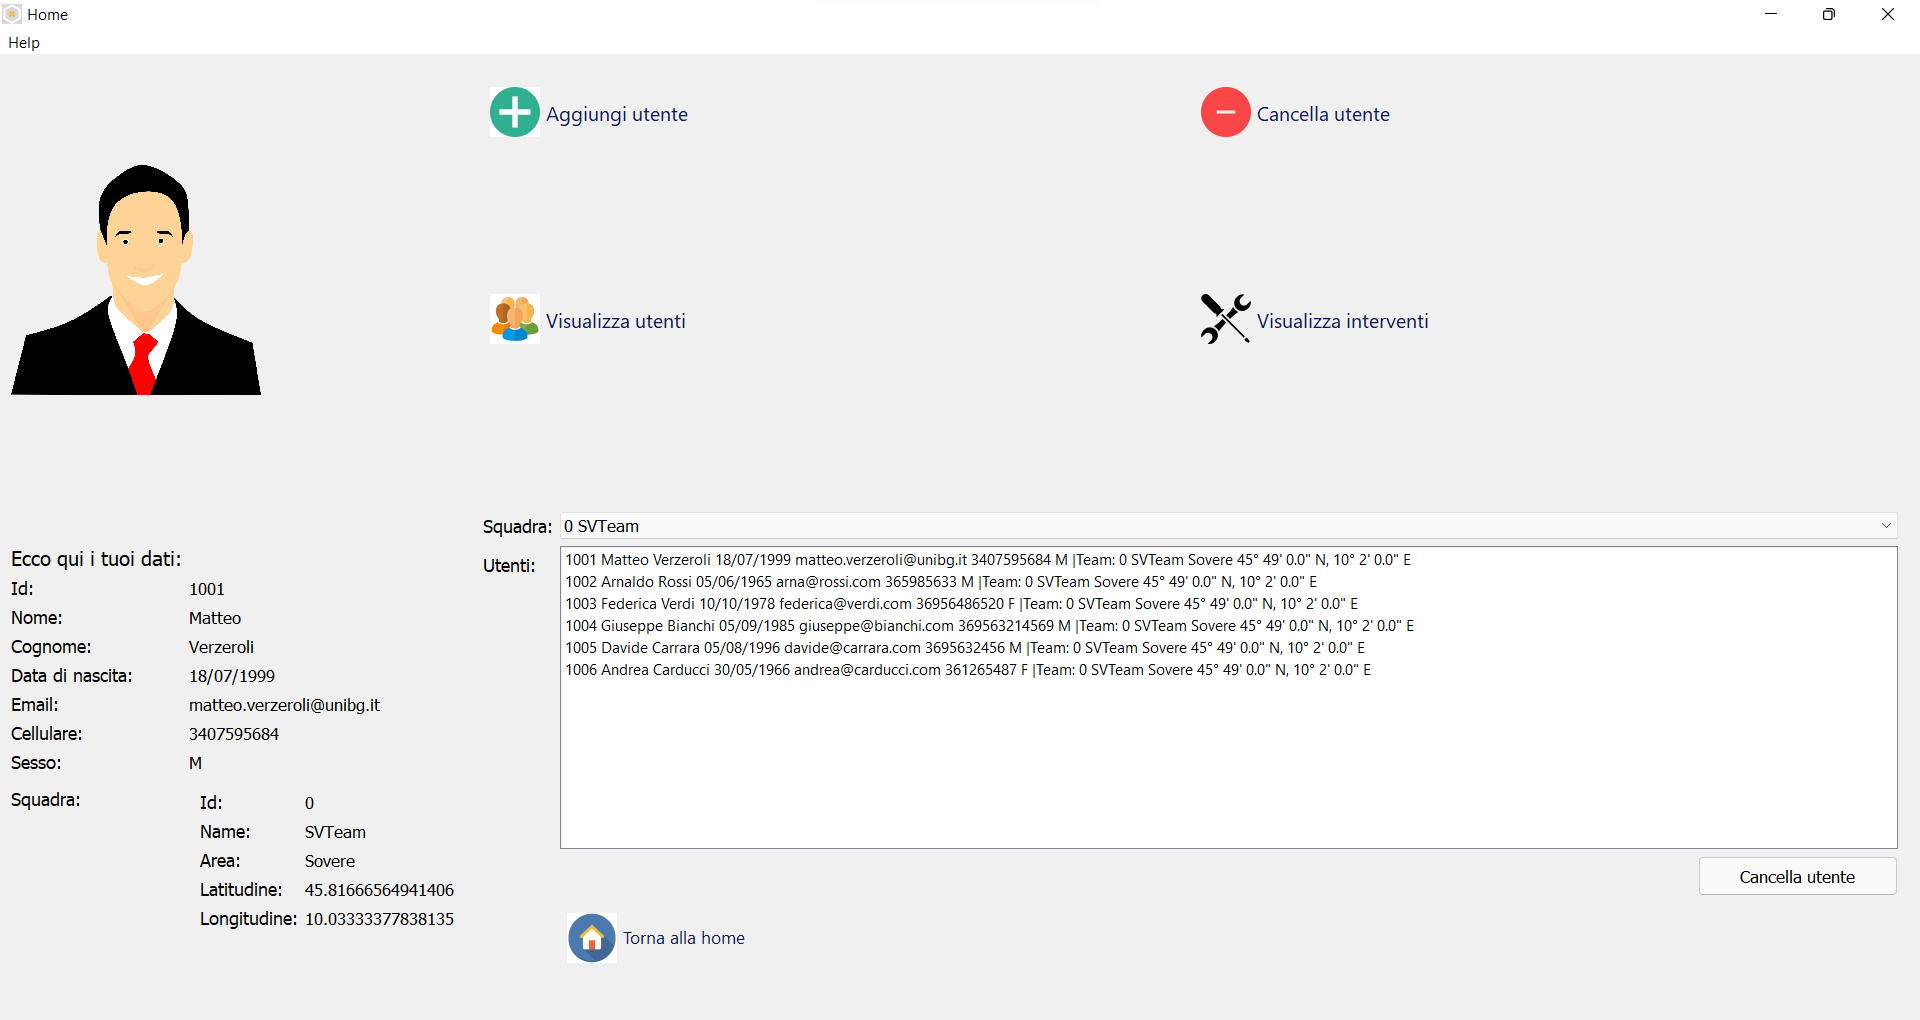
\includegraphics[width=1\linewidth]{./ImageFiles/delete_user}
	\caption{Cancellazione utente.}
	\label{fig:delete_user}
\end{figure}

\subsection{Visualizza utenti}
\subsection{Visualizza interventi}

\begin{landscape}
	\section{Diagramma delle classi}
	\begin{figure}[h!]
		\centering
		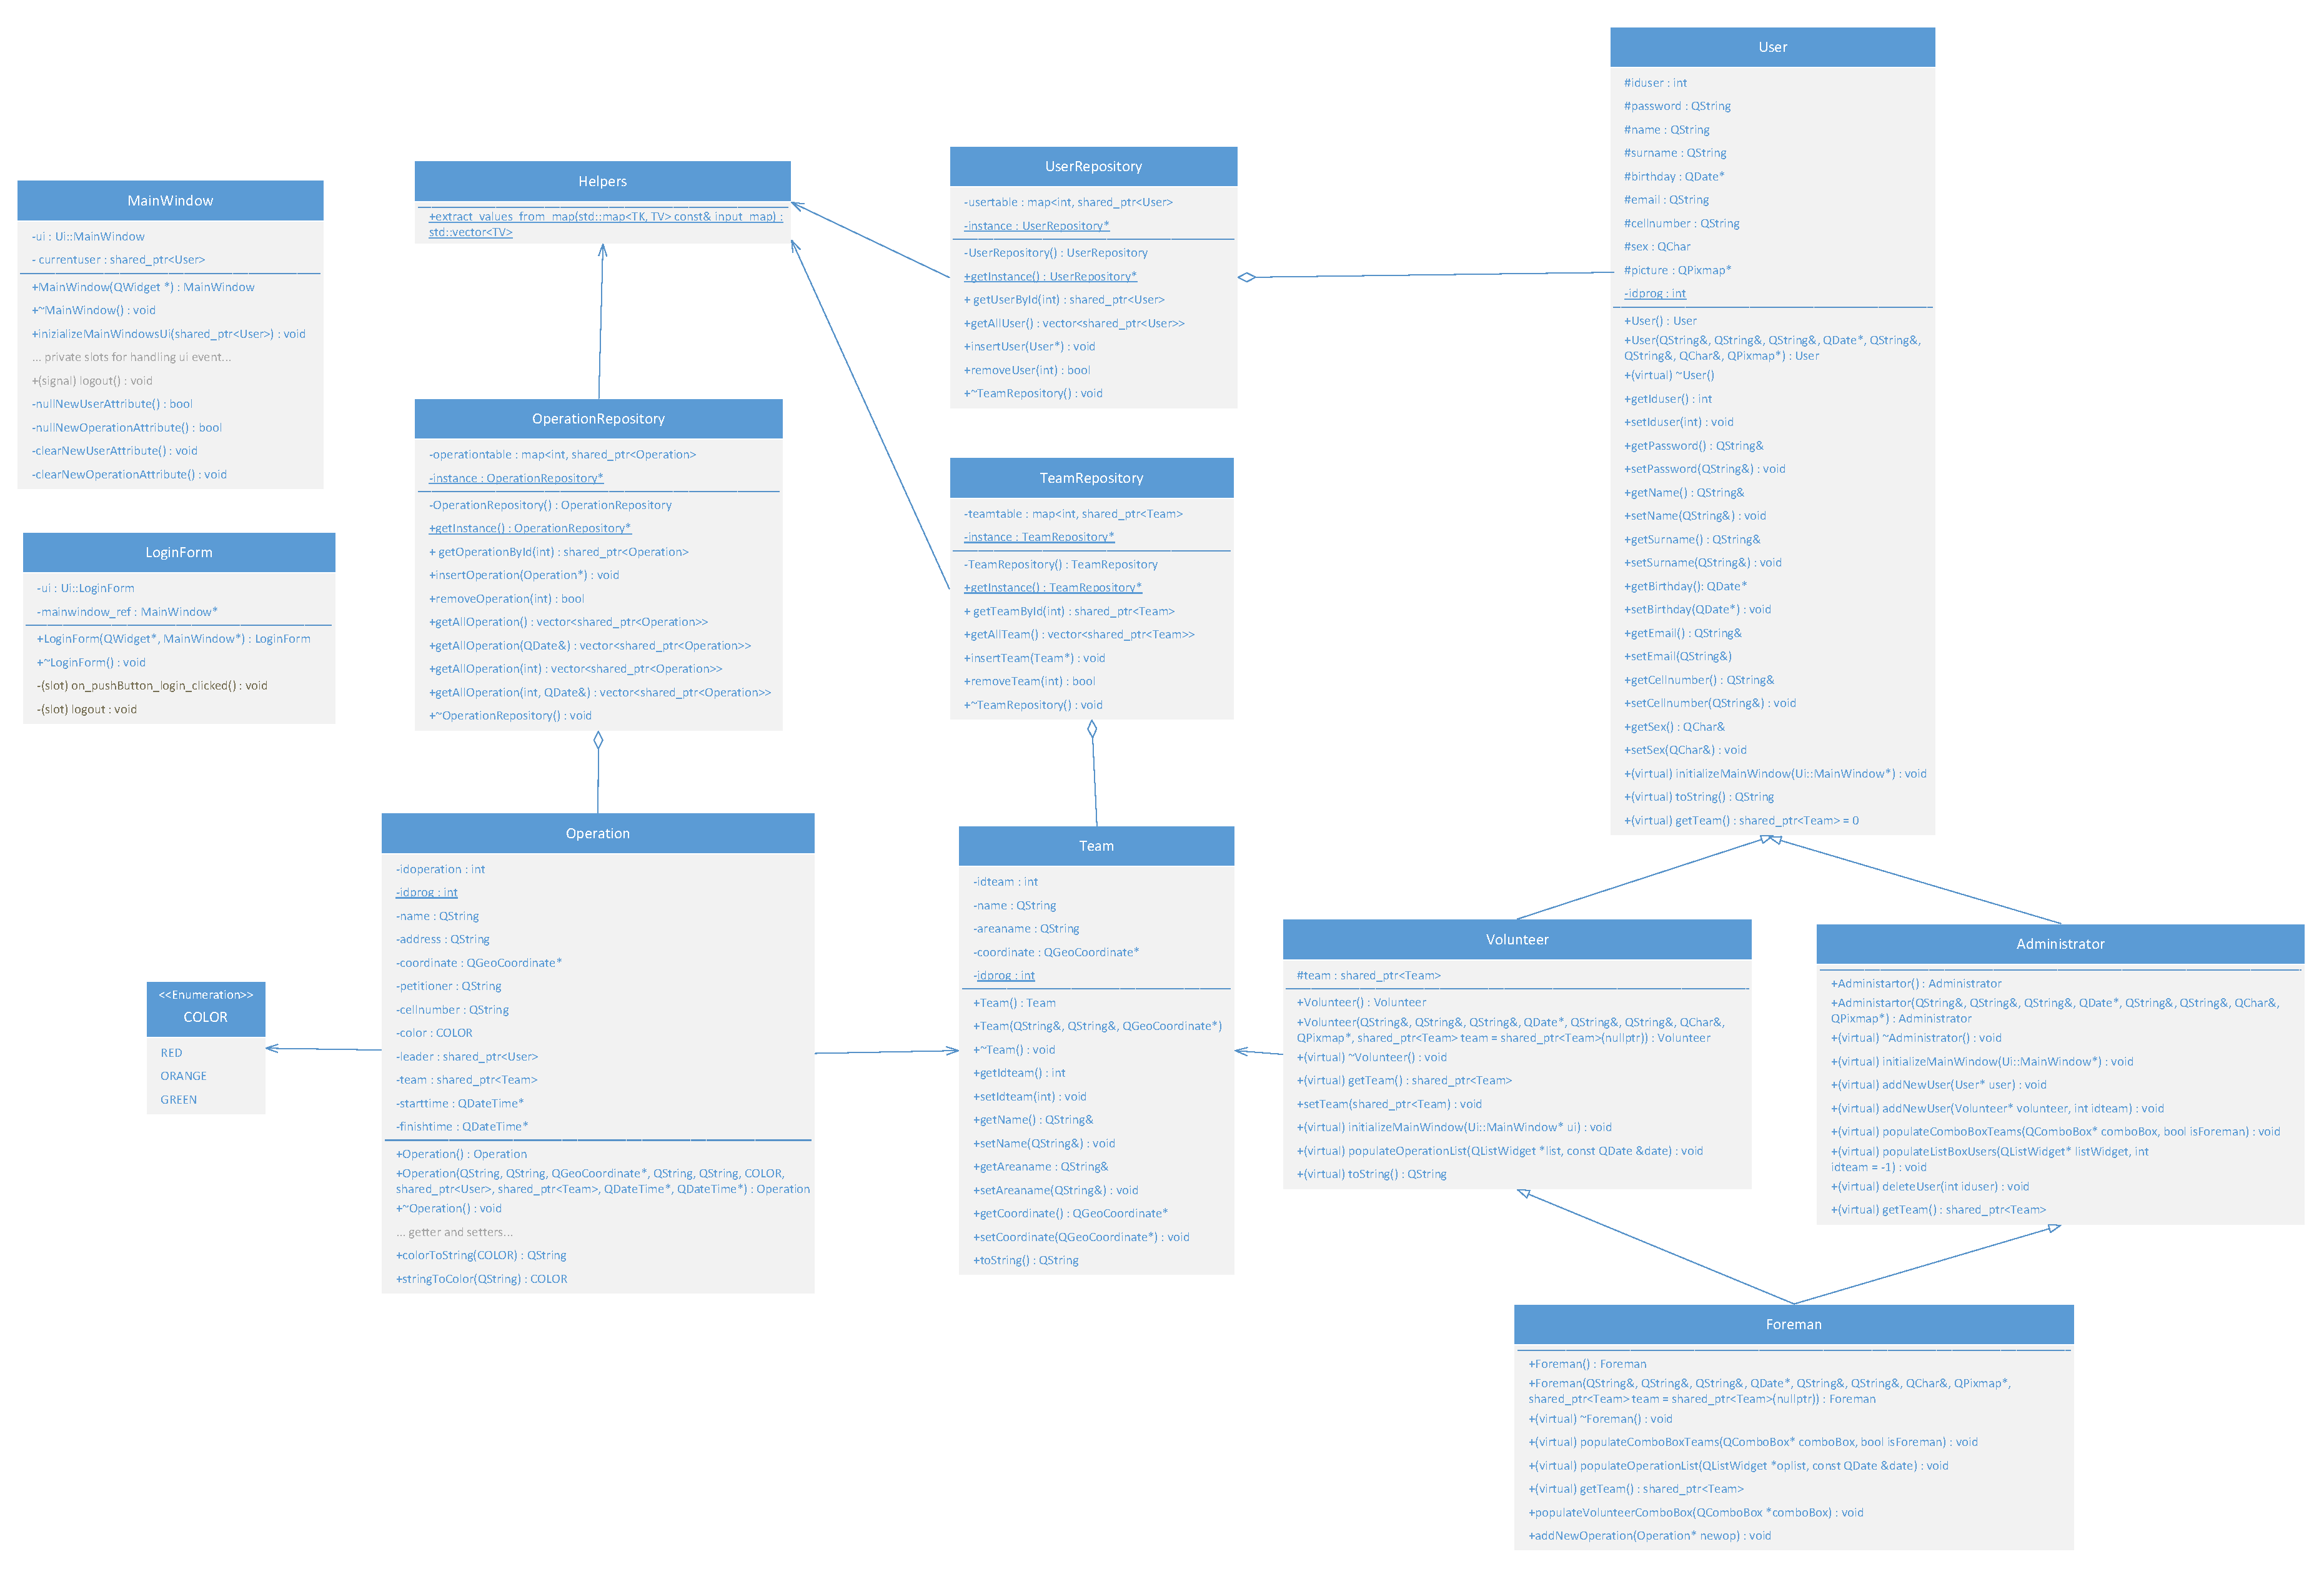
\includegraphics[width=0.7\linewidth]{./OtherFiles/Class Diagram}
		\caption{Class Diagram.}
		\label{fig:class_diagram}
	\end{figure}
\end{landscape}